\chapter{Proposed Method}
\section{Intorduction}
First of all, we can see a basic idea of our research from Figure. \\
\begin{figure}[!hbp]
\centering
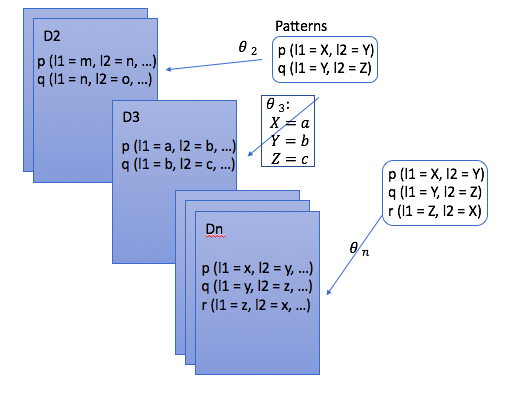
\includegraphics[width=250pt]{./pictures/0301.png}
\caption{Image of extracting descriptive patterns from document set}
\end{figure}
\\
Structural similarity is a kind of similarity that can be explained by a pattern having a special structure, for example, it includes similarity of graphs. We want to find out a descriptive pattern that can be embedded into some event graphs of the precedents. We can think that it is one kind of evaluation of the distance of graphs, it becomes a problem of data mining. To extract descriptive patterns, we need to extract all candidates first. And the re-construct of the descriptive pattern will be a difficult task.\\
In the following sections, we will discuss our idea and a specific algorithm to re-construct the descriptive patterns. In Section 2, we will talk about some basic definitions, which are very useful for our research. In Section 3, we will introduce what the Descriptive Pattern is. Then we will talk about the importance of nouns and cases. Finally, in Section 6, we will propose an idea to re-construct the Descriptive Pattern.